\documentclass{article}
\usepackage{longtable}
\usepackage{graphicx}

\begin{document}
\section*{Supplemental Information}

\section{Validity of Fatal Encounters between 2000 and 2018}

\subsection{Internet news and Fatal Encounters coverage}

Fatal Encounters data is available for cases between 2000 and 2019, with new cases being added to the dataset on an ongoing basis. Here, we consider whether Fatal Encounters provides reliable data on counts of deaths involving police across the full period included in the dataset. 

We suspect that the data undercount police-involved deaths in periods prior to 2007. In conversation with the authors, the primary collector of the Fatal Encounters data, D. Brian Burghart, believes that the lack of local online news publication, as well as the routine practice of purging archived internet content prior to the advent of inexpensive cloud storage, leads to a significant undercount of cases between 2000 and 2007.

While we were unable to locate time series data on online news consumption or content production for a time series that included the period under consideration, we believe that data on general internet usage among the US population should correlate with these variables. We obtain time series data on the rates of internet usage among US adults from the St. Louis Federal Reserve (World Bank, Internet users for the United States [ITNETUSERP2USA], retrieved from FRED, Federal Reserve Bank of St. Louis; https://fred.stlouisfed.org/series/ITNETUSERP2USA, February 15, 2019.), and compare this data to counts of police-involved deaths derived from Fatal Encounters by year in Figure \ref{fig:internet}

\begin{figure}
	\centering
	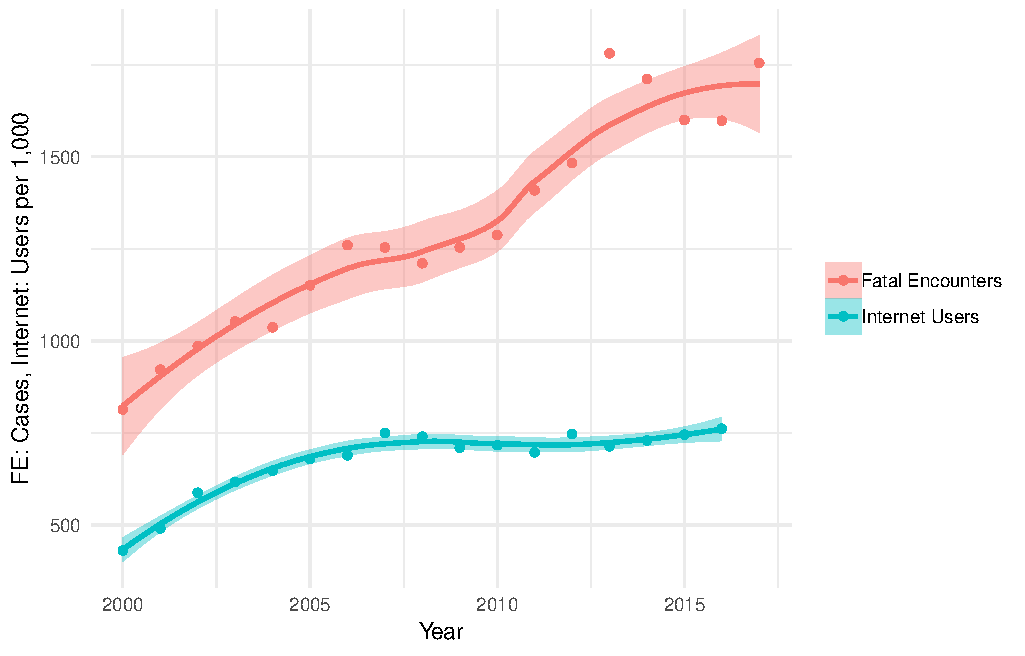
\includegraphics[width=\linewidth]{vis/internet_use_ts.pdf}
	\caption{Deaths recorded in Fatal Encounters and Internet users per 1,000 persons, 2000 to 2016.}
	\label{fig:internet}
\end{figure}

Figure \ref{fig:internet} shows a close correlation between the increasing use of the internet among Americans and the counts of deaths recorded in Fatal Encounters for the years 2000 through 2007. The trends appear to decouple after 2007. This is consistent with a censorship hypothesis. In earlier years of the data, there is likely a larger unobserved set of cases that are not accessible to Fatal Encounters researchers using their web-based search methodology than there is in later years of the data. 

\subsection{Comparing trends in NVSS and Fatal Encounters}

Prior research has established that the National Vital Statistics System systematically undercounts officer-involved deaths (CITES). However, assuming that there have been no changes in the probability that officer-involved deaths would be coded as legal intervention deaths in NVSS over time, the observable time series trends in NVSS should be correlated with the true unobserved count of police-involved deaths. With this assumption, we can evaluate the time series of NVSS police-involved deaths and Fatal Encounters officer use-of-force deaths to further evaluate the possibility of censorship and gain insight into possible temporal trends in the risk of police-involved death. We display this time series in Figure \ref{fig:countTS}. Because NVSS under-reports officer-involved deaths, we provide a scaled time series in Figure \ref{fig:pctTS} to enable direct comparison of the two trends on a common scale. 

\begin{figure}
	\centering
	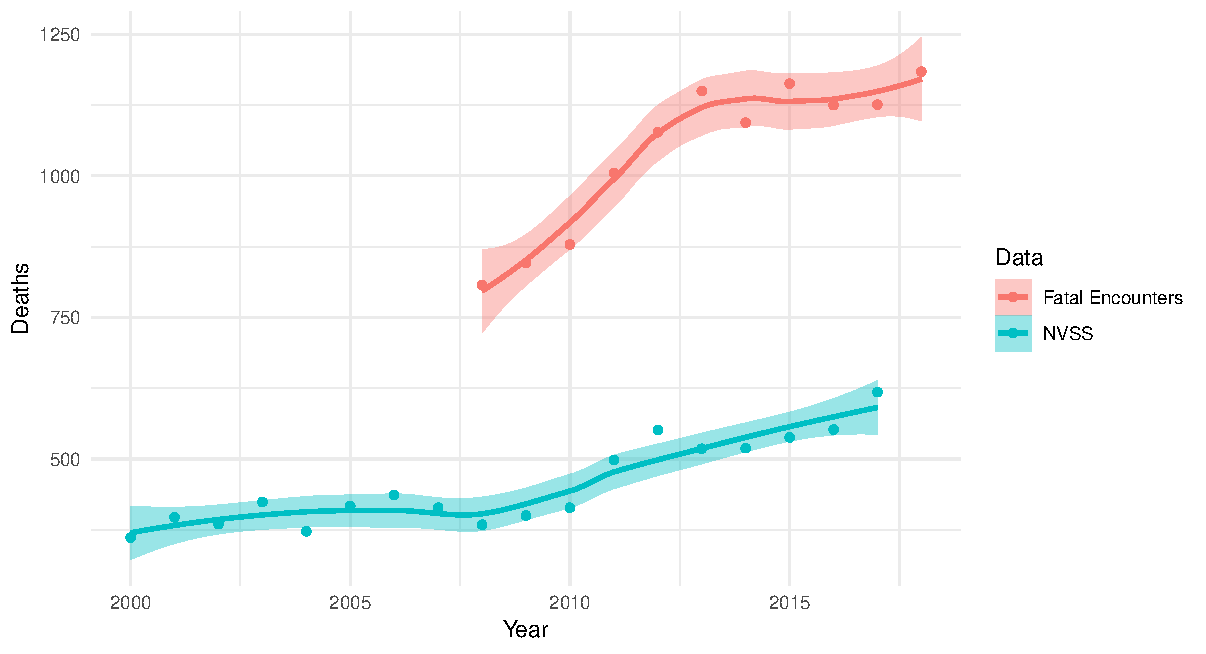
\includegraphics[width = \linewidth]{vis/nvss_fe_ts.pdf}
	\caption{Deaths due to officer use of force recorded in Fatal Encounters and NVSS 2000 to 2018}
	\label{fig:countTS}
\end{figure}

\begin{figure}
	\centering
	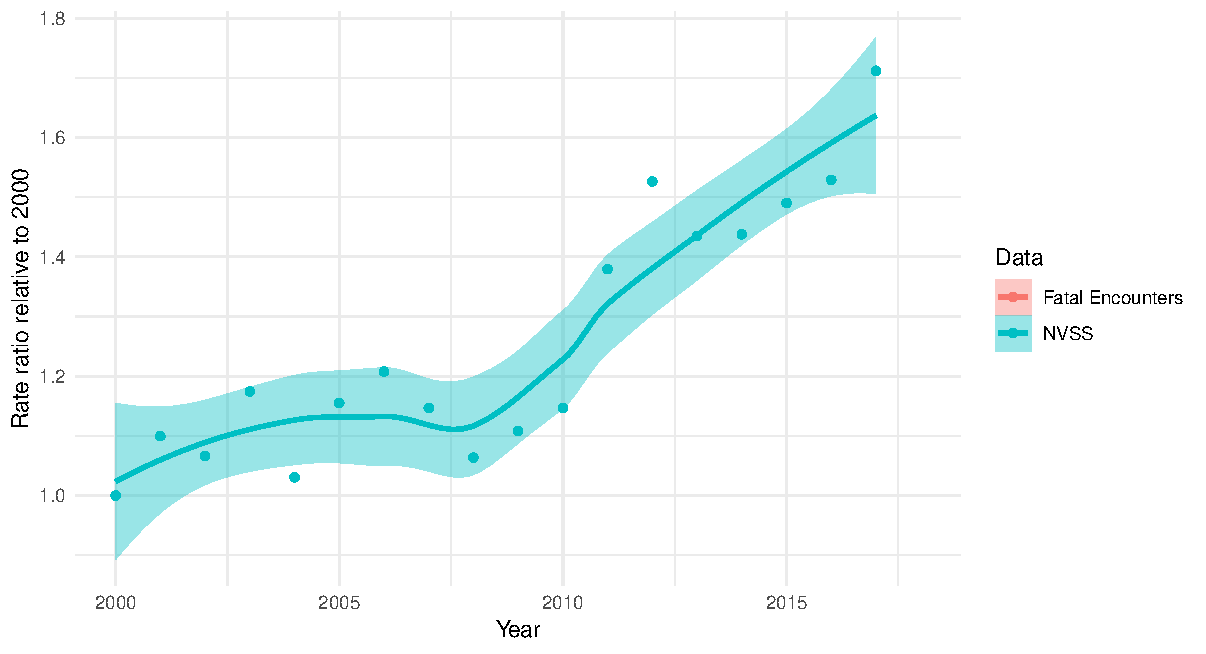
\includegraphics[width = \linewidth]{vis/nvss_fe_pct.pdf}
	\caption{Proportional change in reported deaths in NVSS and Fatal Encounters since 2000}
	\label{fig:pctTS}
\end{figure}

Figures \ref{fig:countTS} and \ref{fig:pctTS} show that counts of deaths reported in NVSS remained relatively stable between 2000 and 2010. During this time, rates fluctuated between 1.0 and 1.2 times the count of officer-involved deaths reported in 2000. Between 2011 and 2017 (the most recent available data), the count of cases in the data increased substantially. In 2017, there were about 1.7 times more legal intervention deaths reported in NVSS than there were in 2000. 

Fatal Encounters exhibits a relatively stable positive trend between 2000 and 2018. The magnitude of growth in cases recorded in FE over time is higher than for NVSS; for 2018, FE records about 2.3 times more deaths than it records for 2000. While this evidence is far from definitive, trends in the proliferation of internet access and the NVSS time series suggest that undercounts in Fatal Encounters due to unavailable online news records of officer-involved deaths likely decreased over time until approximately 2007. The shape of trends in Fatal Encounters and NVSS become more tightly linked between 2008 and 2017. This is consistent with the appraisals of Fatal Encounters' researchers. 

Figure \ref{fig:pct_08} rescales both time series to display proportional changes in case counts relative to the observed counts for 2008. This figure strongly suggests that the trends in NVSS and Fatal Encounters converge after 2008. It may be fruitful in future research to estimate the magnitude of undercoverage in FE using secondary data to provide information on the shape of temporal change in the risk of police-involved killings. Based on this analysis, in this paper we assume that undercoverage in Fatal Encounters becomes less pronounced after 2007, and focus our analyses on cases recorded as occurring between 2008 and 2018. 

\begin{figure}
	\centering
	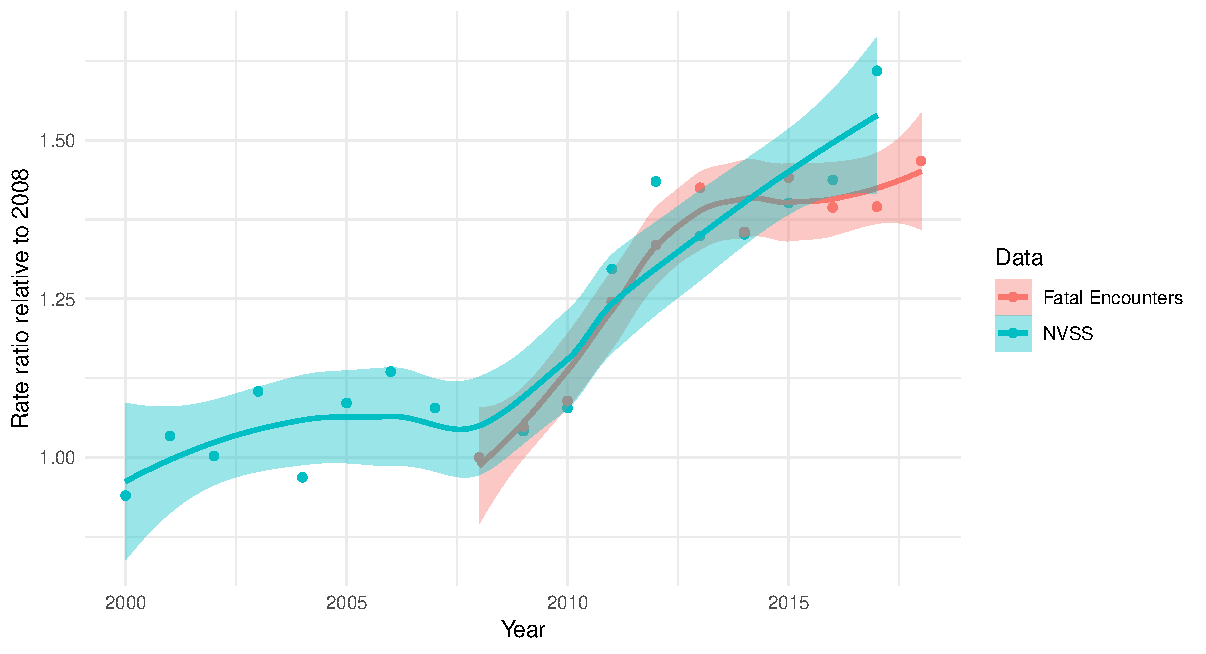
\includegraphics[width = \linewidth]{vis/nvss_fe_pct_08.pdf}
	\caption{Proportional change in reported deaths in NVSS and Fatal Encounters since 2008}
	\label{fig:pct_08}
\end{figure}

\section{Validity of period-stable risk for subgroups}

As shown in figure \ref{fig:pct_08}, there has been an increase in police-involved killings between 2008 and 2018. 

SAY MORE ON LIFE TABLE ASSUMPTIONS ON RISK - ASSUMPTION ISNT THAT RISK IS STABLE, BUT THAT AGE-RISK PATTERNS ARE STABLE, RIGHT? THINK HARD ON THIS

This relatively steep increase in the prevalence of police-involved killings may bias our estimates of the lifetime risk of being killed by police

INCLUDE MIKE'S PLOTS. SAY THAT WE'RE MODELING AND SIMULATING TO NET OUT TIME TRENDS FOR NEW TABLES. SHOULD BE MORE ROBUST TO WITHIN-PERIOD CHANGES

\section{Race/ethnicity data in Fatal Encounters}

Fatal Encounters codes decedent race with the mutually exclusive values: African American/Black; Asian/Pacific Islander; European-American / White; Hispanic / Latino; Middle Easter; Native American / Alaskan; and Race unspecified. Ethnicity is not coded separately from race, so no distinctions among ethnic groups (i.e. Black and non-Black Latinx people) are possible using these data. We preserve these categories in all analyses, with the exception of Middle Eastern, which we recode to "White" based on census racial classifications to match population data. 

Fatal Encounters codes race/ethnicity opportunistically based on a series of potential data sources. When available, official records or news reports that explicitly identify a victim's race or ethnicity are used. However, such identifications are rare in news reports, which typically subscribe to style guidelines limiting the use of racial or ethnic categories in their reporting. When explicit identifications are unavailable, Fatal Encounters researchers combine information and photos from original news reports, obituaries, or social media profiles to make qualitative assessments of a victim's race and ethnicity. 

Like overall counts of cases in Fatal Encounters, earlier years recorded in the data are likely subject to diminished quality due to the gradual development of internet news coverage, and the timing of the development of major social media platforms that made photos of individuals not directly included in news stories more widely available. We show a time series of the proportion of cases missing race/ethnicity data in FE in Figure \ref{fig:missing_race_ts}.

\begin{figure}
	\centering
	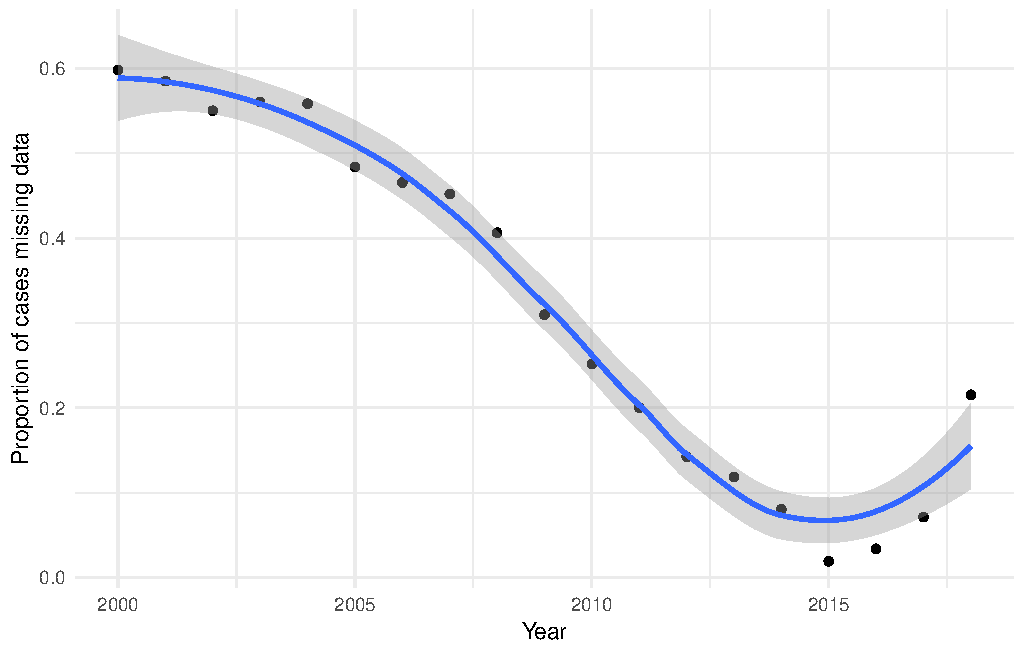
\includegraphics[width=\linewidth]{vis/prop_missing_race.pdf}
	\label{fig:missing_race_ts}
	\caption{Proportion of cases missing data on race/ethnicity in Fatal Encoutners, 2000 - 2018}
\end{figure}

About 60 percent of cases documented for 2000 are missing data on race/ethnicity. This proportion decreases steadily toward a minimum of about two percent of cases in 2015. In 2018, about 20 percent of cases were missing data on race/ethnicity. Fatal Encounters has been unable to code race for many victims prior to 2007 due to the lack of available photos online. The development of online obituaries and the adoption of Facebook increased the availability of searchable photos of victims of police-involved killings. Fatal Encounters researchers also return to cases previously coded only based on news reports to conduct additional searches for obituaries published after the initial incident. In conversation with the authors, Fatal Encounters indicated that missing race/ethnicity data for 2018 and 2019 should be reduced once researchers conduct obituary searches for these years.

\subsection{Comparing Fatal Encounters to NVSS data on race/ethnicity}

NVSS allows us to crudely evaluate the external validity of Fatal Encounters race/ethnicity data through a comparison of the composition of cases in each dataset by identified race/ethnicity. Below, we present the composition of Fatal Encounters cases prior to any missing data imputation procedures to ensure direct comparisons between the data recorded in each source.

\begin{figure}
	\centering
	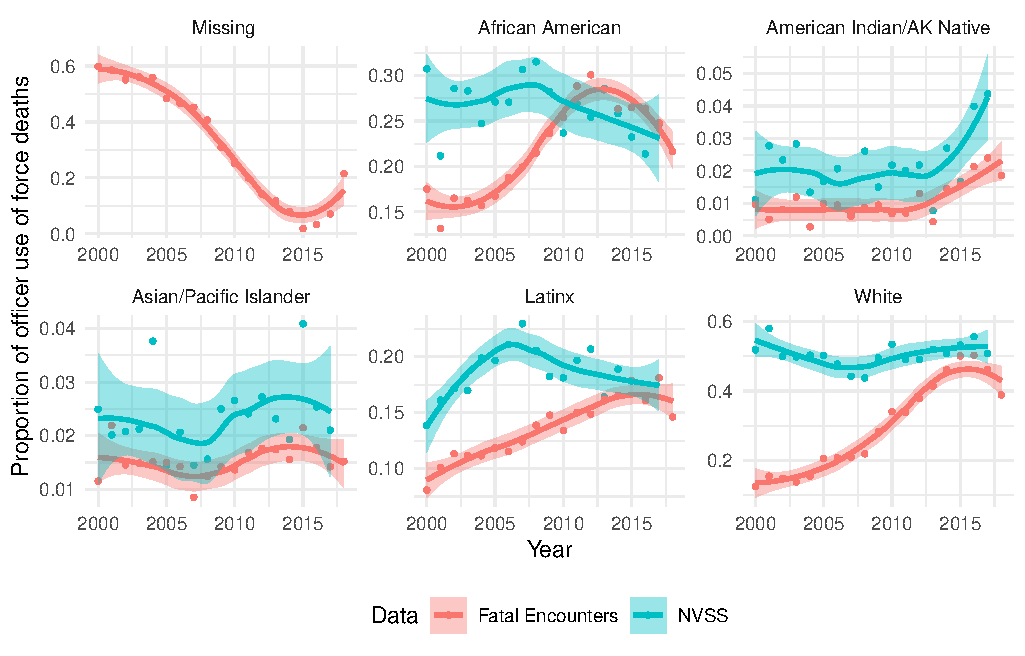
\includegraphics[width = \linewidth]{vis/fe_nvss_race_compare.pdf}
	\caption{Proportion of cases in NVSS and Fatal Encounters by race, including cases missing race/ethnicity data, 2000 - 2018. Note variable scales on y axes}
	\label{fig:compare_missing}
\end{figure}

\begin{figure}
	\centering
	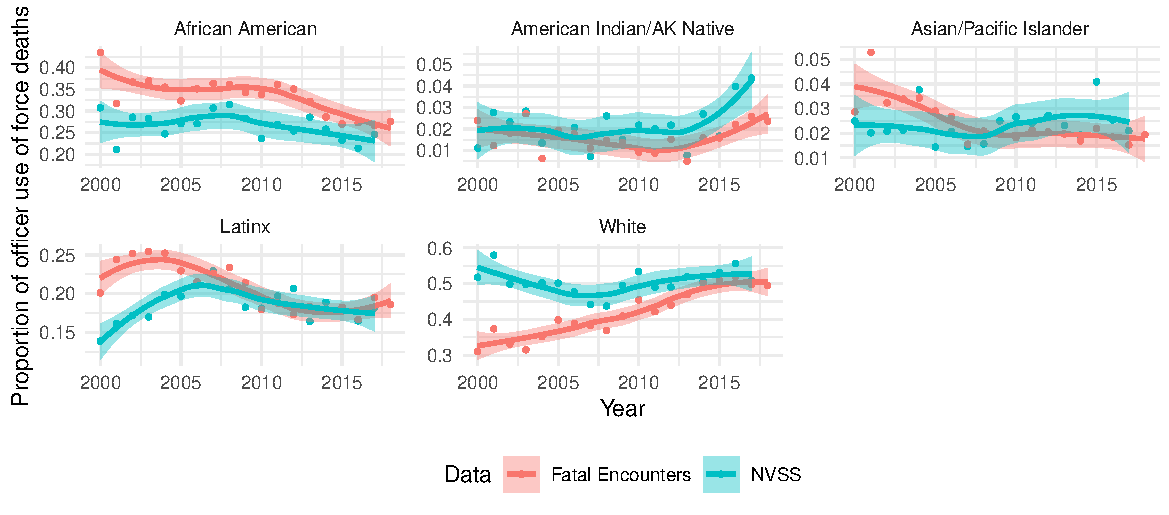
\includegraphics[width = \linewidth]{vis/fe_nvss_race_compare_na_rm.pdf}
	\caption{Proportion of cases in NVSS and Fatal Encounters by race, excluding cases missing race/ethnicity data, 2000 - 2018. Note variable scales on y axes}
	\label{fig:compare_missing_na_rm}
\end{figure}

Figure \ref{fig:compare_missing} shows the composition of cases in each dataset prior to any missing data imputation by race/ethnicity, including missing cases in the total case count. Figure \ref{fig:compare_missing_na_rm} shows the case composition by race/ethnicity \textit{excluding} cases missing race/ethnicity data from the total case count in the proportion denominator. 

Figure \ref{fig:compare_missing_na_rm} shows that both Fatal Encounters and NVSS record similar proportions of American Indian and Alaska Natives and Asian / Pacific Islanders in their total non-missing case compositions. Latinx victims made up a greater share of Fatal Encounters cases prior to 2009; compositions appear similar between 2009 and 2017. African Americans make up a consistently larger share of the case composition in Fatal Encounters than in NVSS. Among non-missing cases, Black victims composed between 40 and 28 percent of the caseload between 2000 and 2018. White victims ranged between 30 and 50 percent of the cases. NVSS consistently reports a white case composition of between 45 and 60 percent. 

As shown in Figures \ref{fig:compare_missing} and \ref{fig:missing_race_ts}, missing data on race in Fatal Encounters is at a minimum between 2012 and 2017. During these years, the relative proportion of victims in all groups recorded in Fatal Encounters is more similar to the proportion recorded in NVSS than it is in earlier years recorded in the data. 

\section{Addressing uncertainty in age-race-sex specific mortality estimates}

For the years 2008 through 2018, we focus on two potential sources of uncertainty in mortality estimates. Missing data, particularly missing data on race/ethnicity suppresses race-specific mortality rates. Estimates that rely on listwise deletion of missing race/ethnicity data would understate underlying mortality risk and would understate uncertainty in underlying mortality risk. 

A second source of uncertainty arises due to the relative rarity of police-involved killings at the age-race-sex specific level. For some groups, national population sizes relative to the probability of the event lead to unstable estimates when we rely on the observed data alone. Model-based simulation can address this problem. We construct statistical models of age-race-sex specific mortality using each imputed dataset, then simulate frequencies of death with larger than observed and standardized population sizes. This approach allows us to quantify uncertainty in mortality risk driven by the combination of small population and rare event features of subgroup specific mortality risk. 

Combining these two approaches, we draw mortality risk uncertainty intervals from regression model posterior distributions estimated on each imputed dataset. This approach jointly accounts for uncertainty and instability resulting from missing data and small population-rare event estimation problems. 

\subsection{Multiple imputation of missing data in Fatal Encounters}

Table \ref{tab:pct_var} shows the percent of cases missing data on each variable in Fatal Encounters between 2008 and 2018 for all causes of death, including suicides and non-use-of-force related deaths. Because we have reason to believe that case counts are censored in earlier years of the data, we exclude observations from 2000 to 2007 in imputation models. About 3 percent of cases are missing data on victim age, about 0.3 percent are missing data on victim sex, about 34 percent are missing data on victim race, and less than one percent are missing data on the cause of death. As shown in Figure \ref{fig:missing_race_ts}, the probability that a case is missing race/ethnicity data is, in part, conditional on the year of the observation. 

% latex table generated in R 3.5.2 by xtable 1.8-3 package
% Wed Mar  6 19:46:07 2019
\begin{table}[ht]
\centering
\begin{tabular}{rrrr}
  \hline
Age & Sex & Race & Cause of death \\ 
  \hline
3.050 & 0.349 & 21.200 & 0.006 \\ 
   \hline
\end{tabular}
\caption{Focal variables missing values in Fatal Encounters, percent of cases 2008 - 2018} 
\label{tab:pct_var}
\end{table}


To address missing data, we draw multiple imputations of missing values in Fatal Encounters based on models including information on the year of death, victim age, victim sex, victim race, the cause of death, the racial composition of the county in which the victim was killed, and the probability of a victim's race/ethnicity conditional on victim surname (compiled from Census surname lists by Imai and Khana (CITE)). Sensitivity analyses exploring the predictive validity of county, tract and block-group-level demographics suggested that county-level demographics maximized model classification validity. This is perhaps due to the fact that geodata recorded in Fatal Encounters records the location of death, and many victims recorded in Fatal Encounters did not die at home. Home addresses would provide greater utility in predicting victim race/ethnicity, but are not available. 

Multiple imputation enables us to model uncertainty in the composition of cases in Fatal Encounters driven by missing data through the construction of uncertainty intervals derived from samples from our missing data models. These estimates are by definition equal to or greater than those directly estimated from the observed data. However, by making the assumption that values are missing at random conditional on the multinomial regression model we use to predict missing values, we are able to provide additional precision in estimating the range within which actual mortality risk lies for each subgroup. Models are estimated using multiple imputation through chained equations (CITE VAN BUUREN). We construct 50 imputed datasets to ensure adequate coverage of uncertainty intervals for the race variable, which has a high share of missingness in earlier years of the data. 

Figure \ref{fig:traceplot} shows the estimated mean and standard deviation of each imputed dataset (color) by variable across iterations, using an MCMC based approach to imputing predicted values in resulting datasets. The traceplots indicate model convergence, and appear free of any trends. 

\begin{figure}
	\centering
	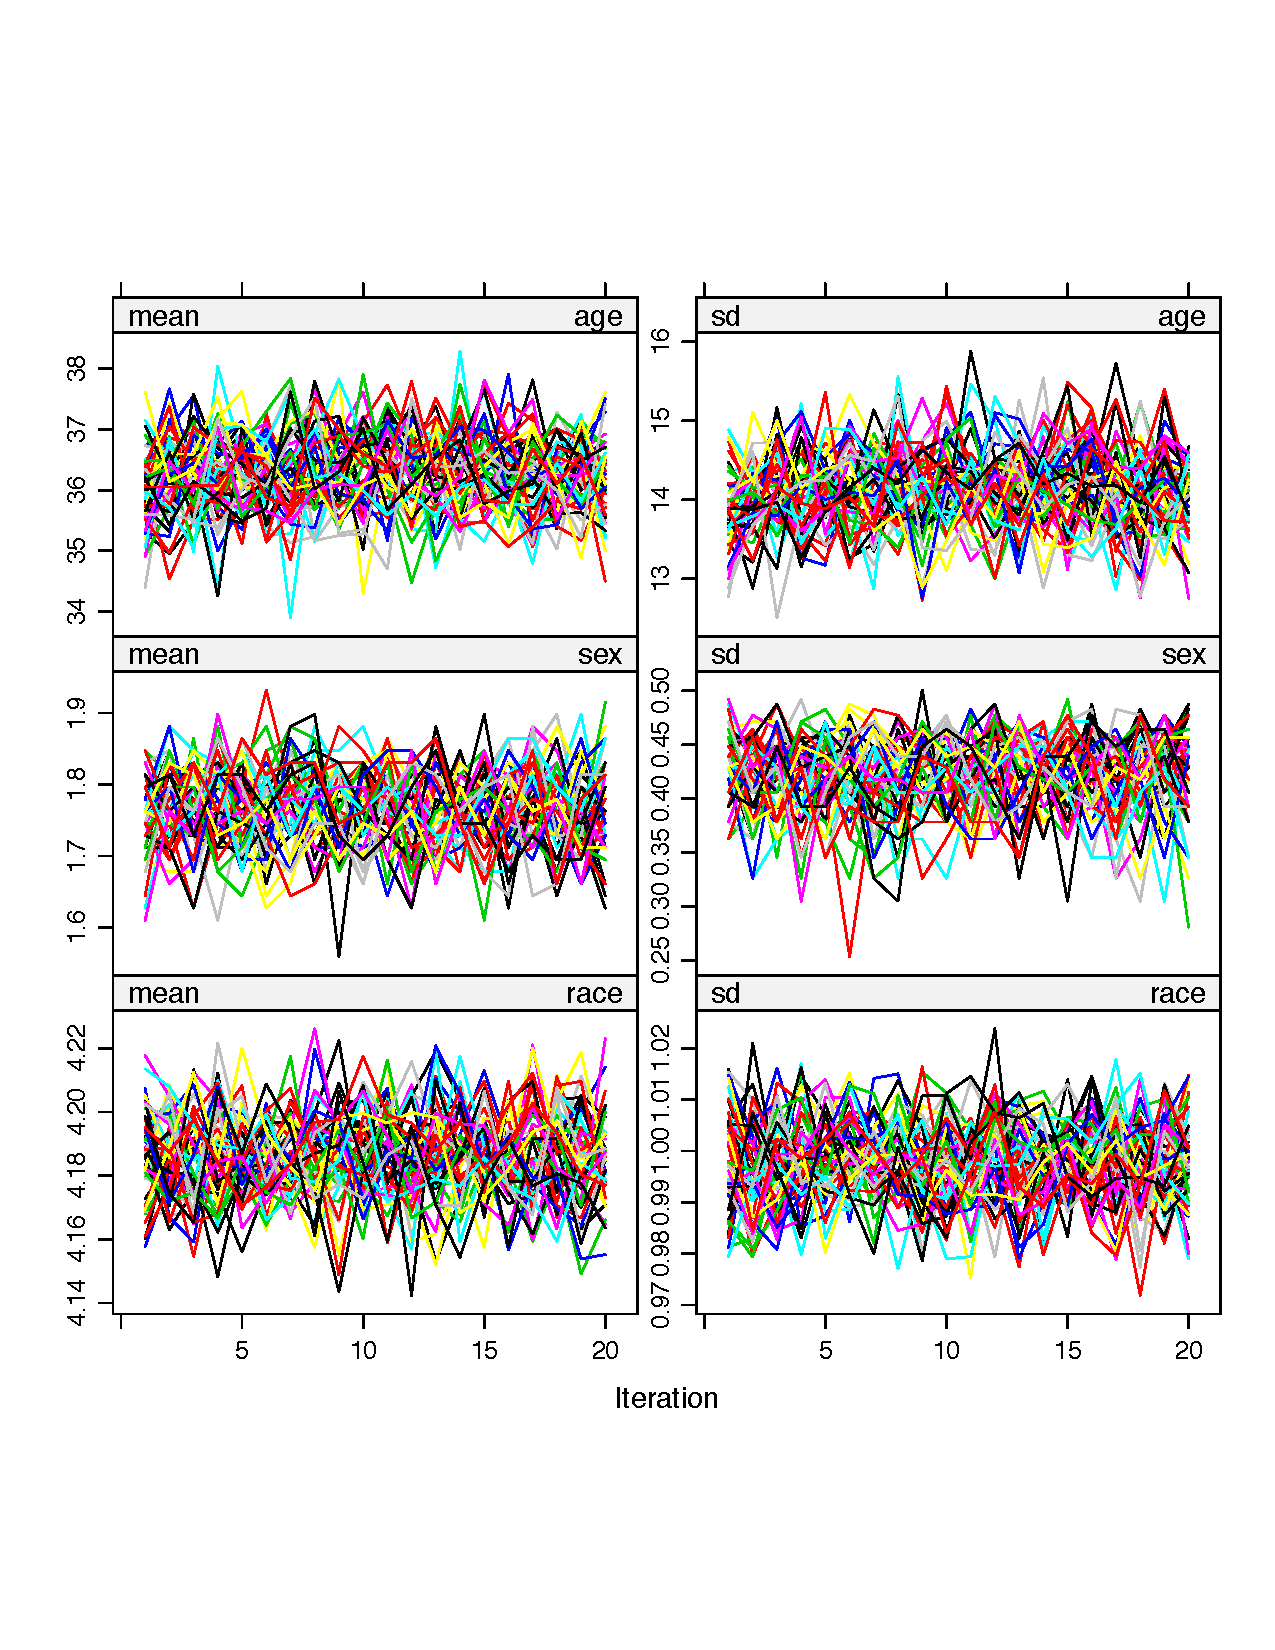
\includegraphics[width = \linewidth]{vis/imp_trace_1.pdf}
	\caption{Traceplot of mean and standard deviation of imputed variables}
	\label{fig:traceplot}
\end{figure}

\begin{figure}
	\centering
	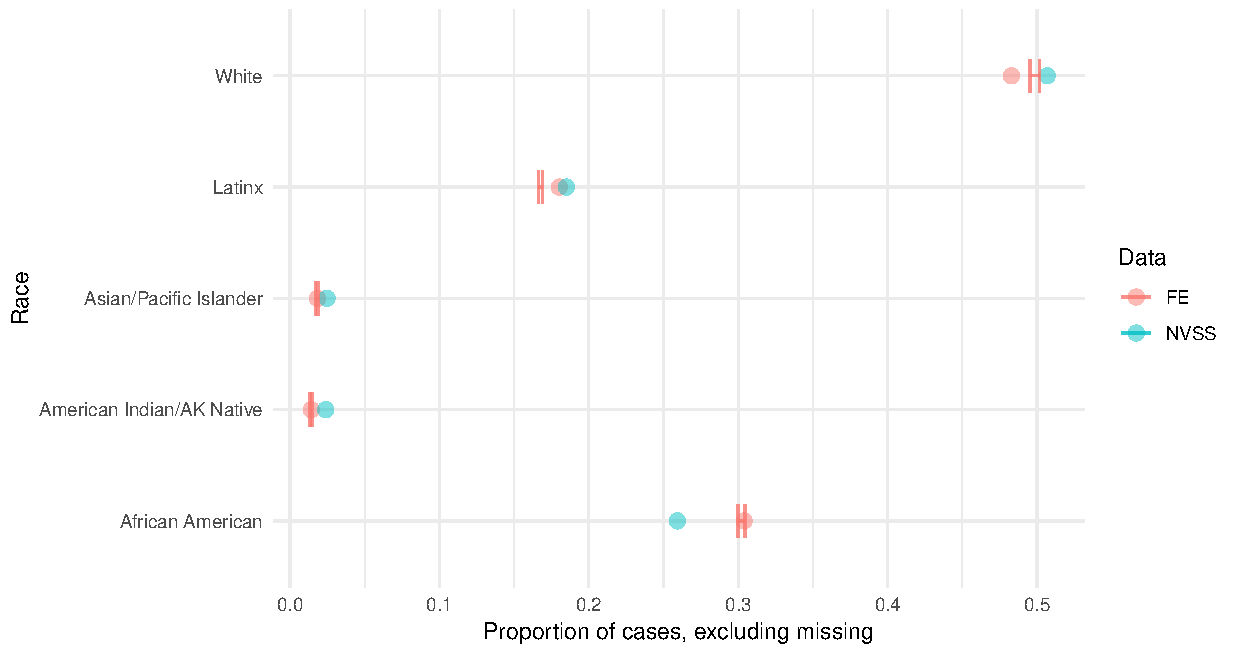
\includegraphics[width = \linewidth]{vis/race_impute_pct.pdf}
	\caption{Proportion of cases in observed Fatal Encounters data (point) and range of imputed data (bar), 2008 - 2018}
	\label{fig:race_impute_pct}
\end{figure}

We show the distribution of the imputed race/ethnicity variable relative to the observed data in Figure \ref{fig:race_impute_pct}. The solid points in this figure represent the observed proportion of cases in each group, and the bars represent the range of the imputed values. For American Indian, Asian, and Black people, the proportion of the observed data in each group is within the range of the imputed values. The distribution of the imputed data do not greatly differ than the distribution of the observed data for these groups. There is a greater share of Latinx victims in the observed data than there are in the imputed data, and there is a greater share of white victims in the imputed data than there are in the observed data. 

In the observed data (excluding missing cases), Latinx victims make up about 18 percent of the recorded cases. Our imputations suggest that they make up between 16.7 and 16.9 percent of all cases. White victims make up about 48 percent of the recorded cases in the observed data. Our imputations suggest they make up between 49.5 and 50.1 percent of all cases. 

This gap between imputed and observed proportions in Fatal Encounters is a function of the relationship between the probability of missingness and a victim's race/ethnicity. Our imputation models address this dependence by including relevant predictors, such as victim surname and population composition in the county of death. 

% latex table generated in R 3.5.2 by xtable 1.8-3 package
% Wed Feb 27 15:47:58 2019
\begin{table}[H]
\centering
\begin{tabular}{lrr}
  \hline
Term & Estimate & SE \\ 
  \hline
County proportion American Indian & 0.20 & 0.45 \\ 
  County proportion Asian & -0.24 & 0.34 \\ 
  County proportion Black & -0.04 & 0.16 \\ 
  County proportion Hispanic & -0.96 & 0.16 \\ 
  Pr(White$|$Surname) & -1.06 & 0.54 \\ 
  Pr(Black$|$Surname) & -0.97 & 0.57 \\ 
  Pr(Hispanic$|$Surname) & -1.16 & 0.54 \\ 
  Pr(Asian$|$Surname) & -0.85 & 0.59 \\ 
   \hline
\end{tabular}
\caption{Relationships between county racial demographics,
         surnames and likelihood of missing race/ethnicity data in Fatal Encounters 2000 - 2018.
         Logistic regression with year intercepts, age slope, sex intercept, and
         cause of death intercept estimated but not displayed.} 
\label{tab:missing_reg}
\end{table}


We evaluate the relationship between the probability that a case is missing and imputation model predictors with a logistic regression model. Selected parameter estimates from this model are displayed in Table \ref{tab:missing_reg}. Cases are less likely to be missing data when they are in counties with large Hispanic populations than when they occur in counties with smaller Hispanic populations. A surname with a high conditional probability of being Hispanic based on census records is also associated with a a lower probability of being missing than is a surname with a high conditional probability of being white. These relationships suggest that names and locations of death are associated with a higher likelihood of positive ethnic identification in Fatal Encounters, either through identifying features in initial reports, or through coder inference based on surname or other contextual information available to coders. Because Latinx victims are less likely to be missing in the observed data, their share of total reports in imputed data is somewhat lower. 

\subsection{Multilevel models of mortality risk and posterior simulation}

\section{Complete life tables}

\end{document}
